\section{Extraction of multipoles}
In order to exctract the multipoles, the structure functions are fitted
with orthogonal Legendre polynomials with $\ell$ up to d-waves:
$$
\begin{array}{l c l}
\sigma_T + \epsilon\sigma_L & = & A_0 + A_1P_0(cos\theta) + A_2P_2(cos\theta) + A_2P_3(cos\theta) + A_3P_4(cos\theta)\\
\sigma_{TT}                 & = & B_0 + B_1P_0(cos\theta) \\
\sigma_{LT}                 & = & C_0 + C_1P_0(cos\theta) + C_2P_2(cos\theta) \\
\end{array}
$$




\begin{figure}[h]
 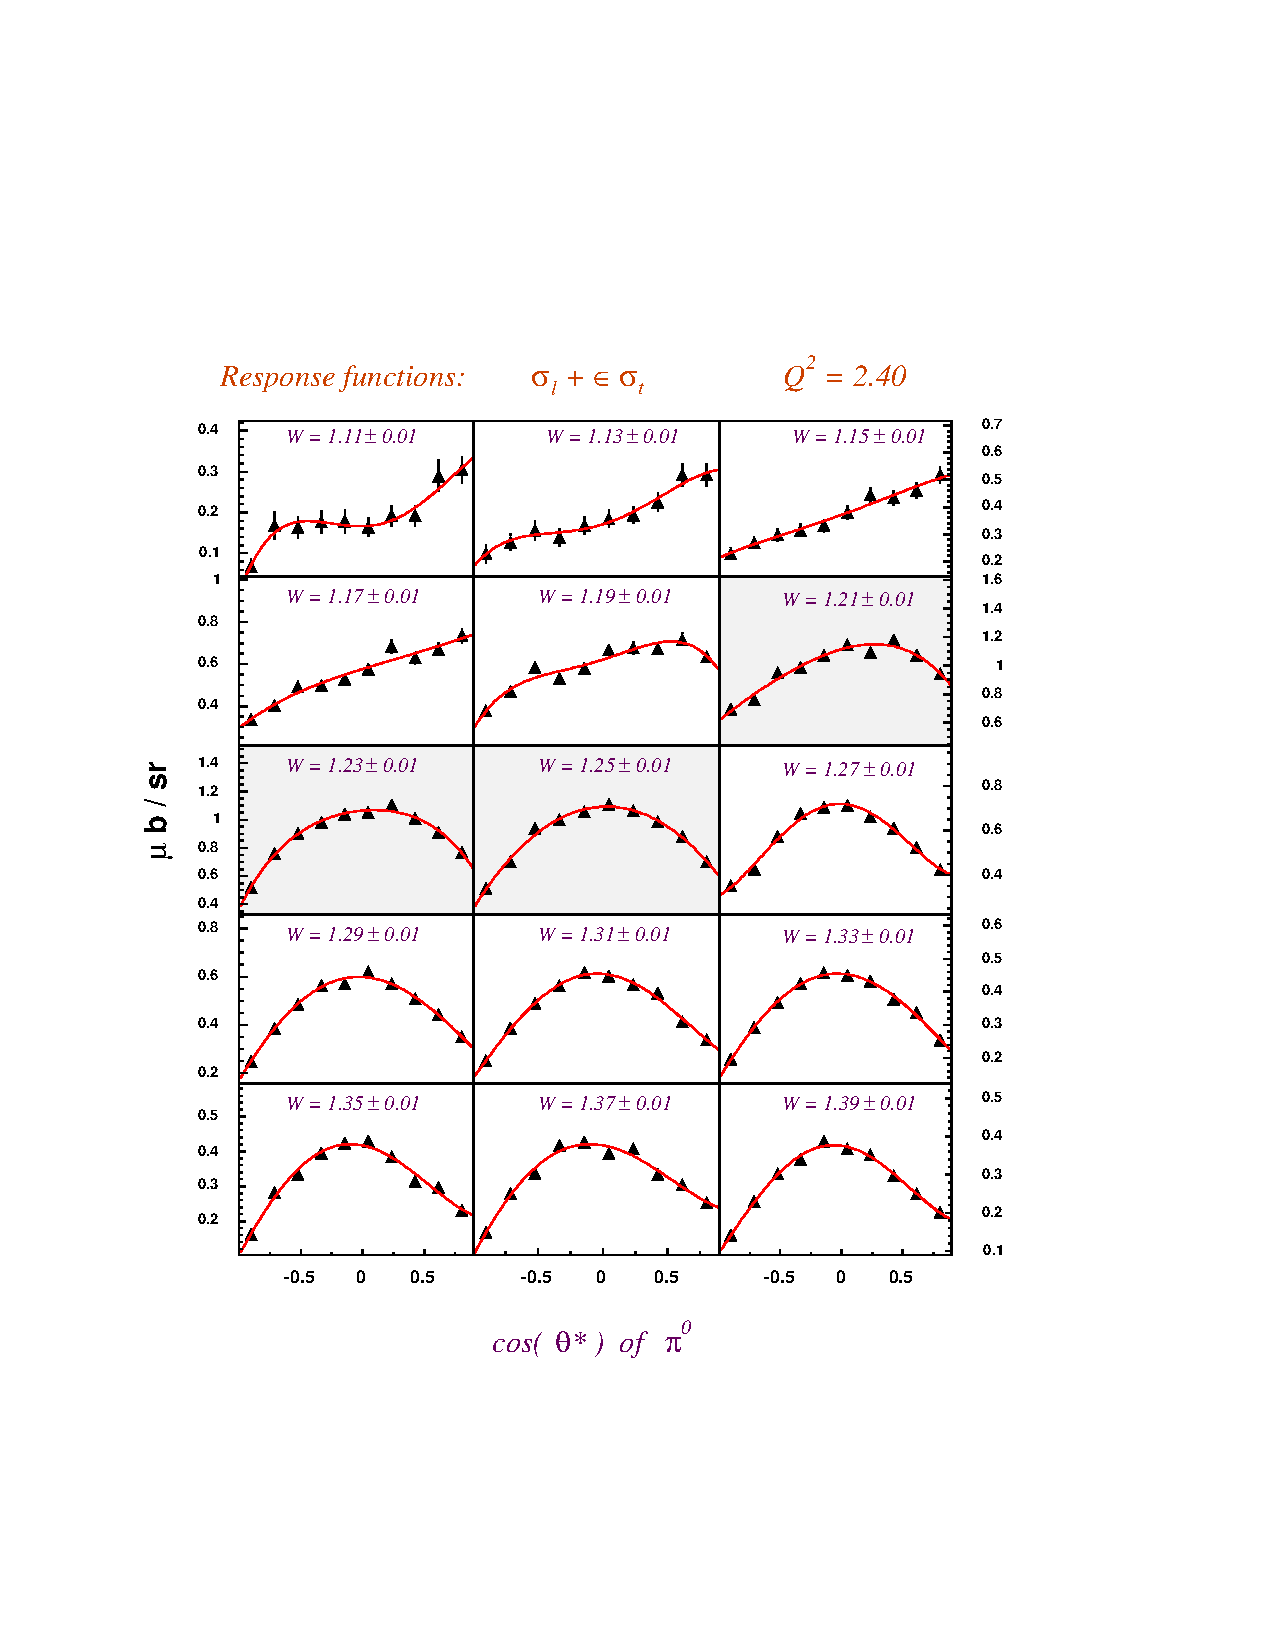
\includegraphics[width = 11cm, bb=60 110 400 640]{analysis/img/Sigma_lpt_Q2_2.40}
  \caption[$\sigma_L + \epsilon\sigma_T$ for different $W$ at $Q^2 = 2.4$ GeV$^2$]
          { $\sigma_L + \epsilon\sigma_T$ for different $W$ at $Q^2 = 2.4$ GeV$^2$. 
	             The highlighted histograms refer to ones used to extract $R_{EM}$ and $R_{SM}$.}
 \label{fig:Sigma_lpt_Q2_2.40}

\end{figure}















